\begin{frame}{Inner Controller}{Linear Quadratic Controller Design}

\only<1| handout:0>
{
  %\item Discrete system representation

  \tikz[overlay,xshift=15em,yshift=1em]{\draw node {
      \begin{minipage}{1\linewidth}
        \begin{figure}[H]
          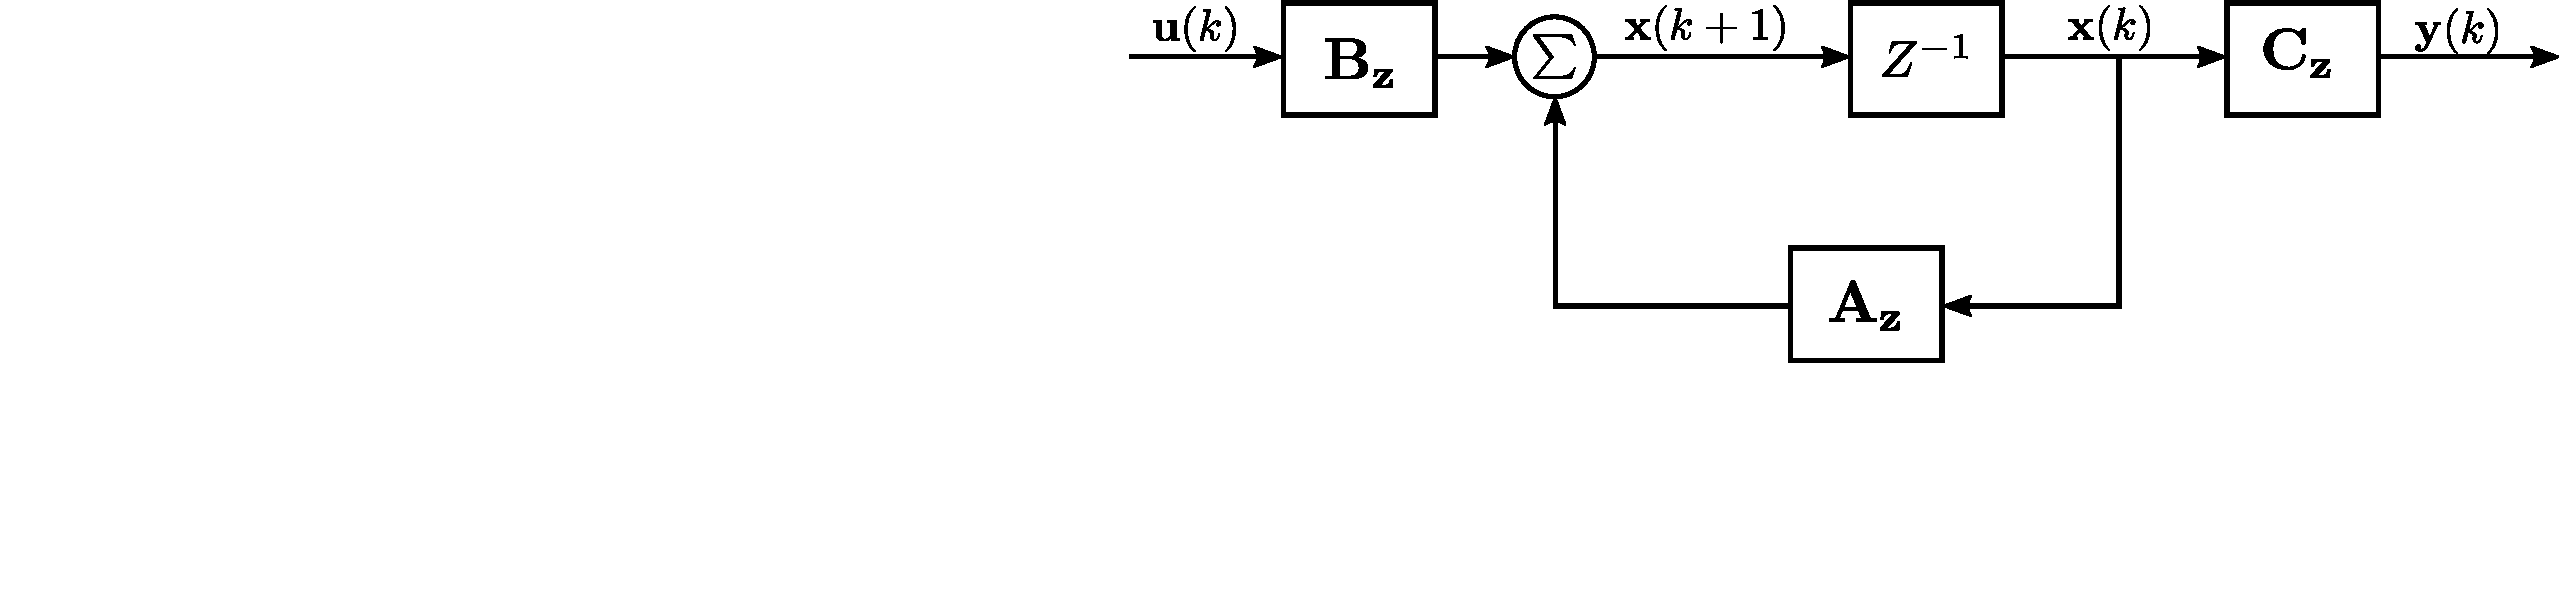
\includegraphics[width=1\textwidth]{figures/LQRblockDiagram1}
        \end{figure}
      \end{minipage}
    };}
  
  
  \tikz[overlay,xshift=12em,yshift=-5em]{\draw node {
      \begin{minipage}{0.01\linewidth}
        \begin{flalign}
          \vec{x}(k+1) &= \vec{A}_z  \vec{x}(k) + \vec{B}_z  \vec{u}(k) \nonumber \\
          \vec{y}(k) &= \vec{C}_z x(k) + \vec{D}_z  \vec{u}(k) \nonumber
        \end{flalign}
      \end{minipage}
  };}
  
}

\only<2-4| handout:1>
{
  %\item Adding a reference
  \tikz[overlay,xshift=15em,yshift=1em]{\draw node {
    \begin{minipage}{1\linewidth}
      \begin{figure}[H]
        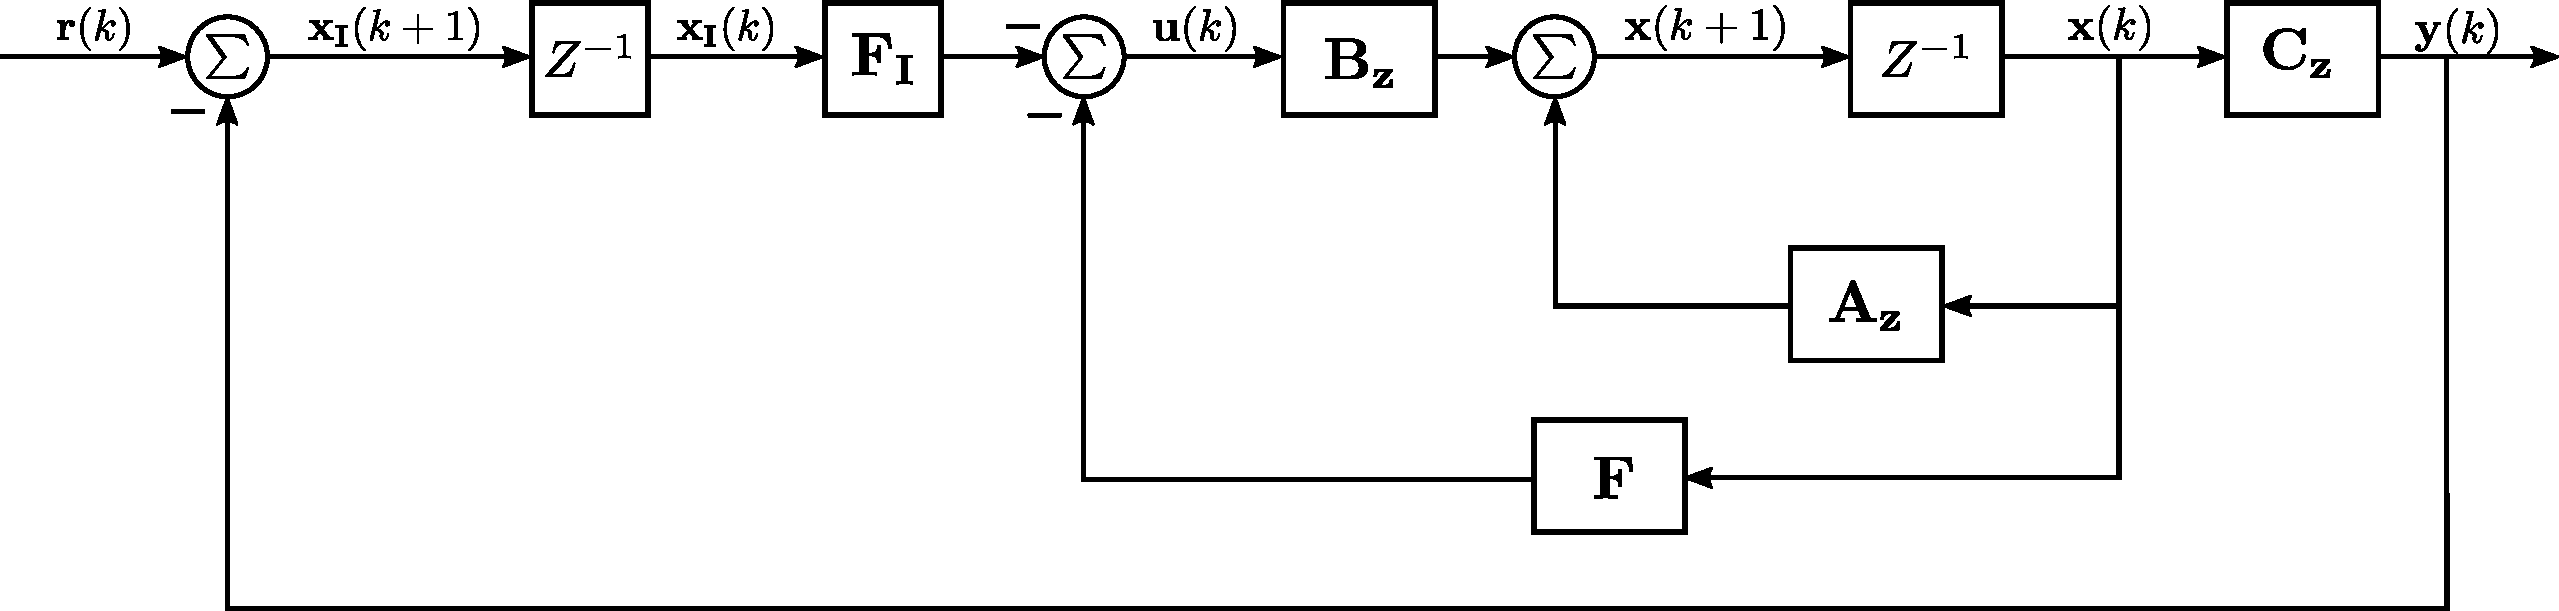
\includegraphics[width=1\textwidth]{figures/LQRblockDiagram2}
      \end{figure}
    \end{minipage}
  };}
}

%\only<0| handout:1>
%{
%  \tikz[overlay,xshift=12em,yshift=-2.5em]{\draw node {
%      \begin{minipage}{0.01\linewidth}
%        \begin{flalign}
%        \vec{x}(k+1) &= \vec{A}_z  \vec{x}(k) + \vec{B}_z  \vec{u}(k) \nonumber \\
%        \vec{y}(k) &= \vec{C}_z x(k) + \vec{D}_z  \vec{u}(k) \nonumber
%        \end{flalign}
%      \end{minipage}
%    };}
%}

\only<2| handout:0>
{
  \tikz[overlay,xshift=12em,yshift=-5.5em]{\draw node {
  };}
}

\only<3| handout:0>
{
  \tikz[overlay,xshift=12em,yshift=-5em]{\draw node {
    \begin{minipage}{0.01\linewidth}
      \begin{flalign}
        \vec{x}_e(k+1) &= \vec{A}_e  \vec{x}_e(k) + \vec{B}_e  \vec{u}(k) + \vec{r}(k) \nonumber \\
        \vec{y}(k) &= \vec{C}_e  \vec{x}_e(k) \nonumber
      \end{flalign}
    \end{minipage}
  };}
}

\only<4| handout:1>
{
  \tikz[overlay,xshift=12em,yshift=-5.5em]{\draw node {
    \begin{minipage}{0.01\linewidth}
      \begin{flalign}
      \hspace{2cm}
        \begin{bmatrix}
          \vec{x}(k+1)  \\
          \vec{x}_\mathrm{I}(k+1)
        \end{bmatrix}
        &=
        \begin{bmatrix}
         \ \ \ \vec{A}_\mathrm{z,3x3} & \vec{0}_\mathrm{3x2} \\
         -\vec{C}_\mathrm{z,2x3} & \vec{I}_\mathrm{2x2} \\
        \end{bmatrix}
        \begin{bmatrix}
          \vec{x}(k)    \\
          \vec{x}_\mathrm{I}(k)
        \end{bmatrix}
        +
        \begin{bmatrix}
          \vec{B}_\mathrm{z,3x2} \\
          \vec{0}_\mathrm{2x2}
        \end{bmatrix}
        \vec{u}(k)
        +
        \begin{bmatrix}
          \vec{0}_\mathrm{3x2} \\
          \vec{I}_\mathrm{2x2}
        \end{bmatrix}
        \vec{r}(k) \nonumber \\ \nonumber \\[-10pt]
        \vec{y}(k)
        &=
        \begin{bmatrix}
          \vec{C}_\mathrm{z,2x3} &  \vec{0}_\mathrm{2x2}
        \end{bmatrix}
        \begin{bmatrix}
          \vec{x}(k)    \\
          \vec{x}_\mathrm{I}(k)
        \end{bmatrix} \nonumber
      \end{flalign}
    \end{minipage}
  };}
}

\end{frame}



\begin{frame}{Inner Controller}{Linear Quadratic Controller Design}

\only<1| handout:0>
{
  \tikz[overlay,xshift=12em,yshift=5.5em]{\draw node {
    \begin{minipage}{0.01\linewidth}
      \begin{flalign}
      \mathcal{J}_\mathrm{z} = \sum_{k=0}^\infty \vec{x}^\mathrm{T}(k)\vec{Q}_\mathrm{z}\vec{x}(k) + \vec{u}^\mathrm{T}(k)\vec{R}_\mathrm{z}\vec{u}(k) \nonumber
      \end{flalign}
    \end{minipage}
  };}
  \tikz[overlay,xshift=12em,yshift=1em]{\draw node {
  };}
  \tikz[overlay,xshift=12em,yshift=-5em]{\draw node {
  };}
}

\only<2-4| handout:1>
{
  \tikz[overlay,xshift=12em,yshift=5.5em]{\draw node {
      \begin{minipage}{0.01\linewidth}
        \begin{flalign}
        \mathcal{J}= \int_{0}^\infty \vec{x}^\mathrm{T}(t)\vec{Q}\vec{x}(t) + \vec{u}^\mathrm{T}(t)\vec{R}\vec{u}(t) \ dt \nonumber
        \end{flalign}
      \end{minipage}
    };}
  \tikz[overlay,xshift=12em,yshift=1em]{\draw node {
    };}
  \tikz[overlay,xshift=12em,yshift=-5em]{\draw node {
    };}
}


\only<1-2| handout:0>
{
  \tikz[overlay,xshift=12em,yshift=1em]{\draw node {
  };}
}

\only<3-4| handout:1>
{
  \tikz[overlay,xshift=12em,yshift=1em]{\draw node {
    \begin{minipage}{0.01\linewidth}
      \begin{flalign} 
        \hspace{2cm}
        Q &= \left(
        \frac{1}{{\psi_\mathrm{max}}\text{}^2} \ , \ 
        \frac{1}{{\dot{\psi}_\mathrm{max}}\text{}^2} \ , \ 
        \frac{1}{{\dot{x}_{b,\mathrm{max}}}\text{}^2} \ , \ 
        \frac{1}{x_{\mathrm{I},\psi,\mathrm{max}}\text{}^2} \ , \ 
        \frac{1}{x_{\mathrm{I},\dot{\psi},\mathrm{max}}\text{}^2} \ , \ 
        \frac{1}{x_{\mathrm{I},\dot{x_b},\mathrm{max}}\text{}^2} \right)
        \nonumber
      \end{flalign}
%      \begin{flalign}
%      \dot{\vec{x}}(t) &= \vec{A}  \vec{x}(t) + \vec{B}  \vec{u}(t) + r(t)\nonumber \\
%      \vec{y}(t) &= \vec{C} x(t)  \nonumber
%      \end{flalign}
    \end{minipage}
  };}
}

\only<1-3| handout:0>
{
  \tikz[overlay,xshift=12em,yshift=-5em]{\draw node {
  };}
}

\only<4| handout:1>
{
  \tikz[overlay,xshift=12em,yshift=-5em]{\draw node {
  \begin{minipage}{0.01\linewidth}
    \begin{flalign}
      \hspace{2cm}
      R &= \left(
      \frac{1}{{{F_1}_\mathrm{max}}\text{}^2} \ , \ 
      \frac{1}{{{F_2}_\mathrm{max}}\text{}^2} \right)
      \nonumber
    \end{flalign}
    \begin{flalign}
      \hspace{2.5cm}
      \vec{u} = - \begin{bmatrix}
                    \vec{F} & \vec{F}_\mathrm{I}
                  \end{bmatrix}
                  \begin{bmatrix}
                    \vec{x}  \\
                    \vec{x}_\mathrm{I}
                  \end{bmatrix}
      \nonumber
    \end{flalign}
%    \begin{flalign}
%      \hspace{2cm}
%      \begin{bmatrix}
%        \dot{\vec{x}}(t)  \\
%        \dot{\vec{x}}_\mathrm{I}(t)
%      \end{bmatrix}
%      &=
%      \begin{bmatrix}
%      \ \ \ \vec{A}_\mathrm{3x3} & \vec{0}_\mathrm{3x2} \\
%       -\vec{C}_\mathrm{2x3} & \vec{I}_\mathrm{2x2} \\
%      \end{bmatrix}
%      \begin{bmatrix}
%        \vec{x}(t)    \\
%        \vec{x}_\mathrm{I}(t)
%      \end{bmatrix}
%      +
%      \begin{bmatrix}
%        \vec{B}_\mathrm{3x2} \\
%        \vec{0}_\mathrm{2x2}
%      \end{bmatrix}
%      \vec{u}(k)
%      +
%      \begin{bmatrix}
%        \vec{0}_\mathrm{3x2} \\
%        \vec{I}_\mathrm{2x2}
%      \end{bmatrix}
%      \vec{r}(t) \nonumber \\ \nonumber \\[-10pt]
%      \vec{y}(t)
%      &=
%      \begin{bmatrix}
%        \vec{C}_\mathrm{2x3} &  \vec{0}_\mathrm{2x2}
%      \end{bmatrix}
%      \begin{bmatrix}
%        \vec{x}(t)    \\
%        \vec{x}_\mathrm{I}(t)
%      \end{bmatrix} \nonumber
%    \end{flalign}
  \end{minipage}
  };}
}
\end{frame}



\begin{frame}{Inner Controller}{Comparison of the Controllers}
  Simulation of LQR and robust design
  \begin{itemize}
    \item<1-> Disturbances from wind and waves
    \begin{itemize}
      \item<1-> $\pm 1.5$ N along $\dot{x}_b$
      \item<1-> $\pm 1.5$ N$\cdot$m around $z_b$
      \item<1-> The frequency for both varies between $0$-$10$ Hz 
    \end{itemize}
    \item<2-> The parameters are varied $\pm 20\%$
    \begin{itemize}
      \item<2-> Mass, $m$
      \item<2-> Moment of inertia, $I_z$, around $z_b$
      \item<2-> The damping coefficients $d_x$ and $d_\psi$
      \item<2-> The lengths $l_1$ and $l_2$
    \end{itemize}
  \item<3-> Monte Carlo simulations with $1000$ realizations
  \end{itemize}
\end{frame}


\begin{frame}{Inner Controller}{Comparison of the Controllers}
\begin{figure}[H]
  \begin{minipage}{0.45\linewidth}
    \begin{figure}[H]
      \centering
      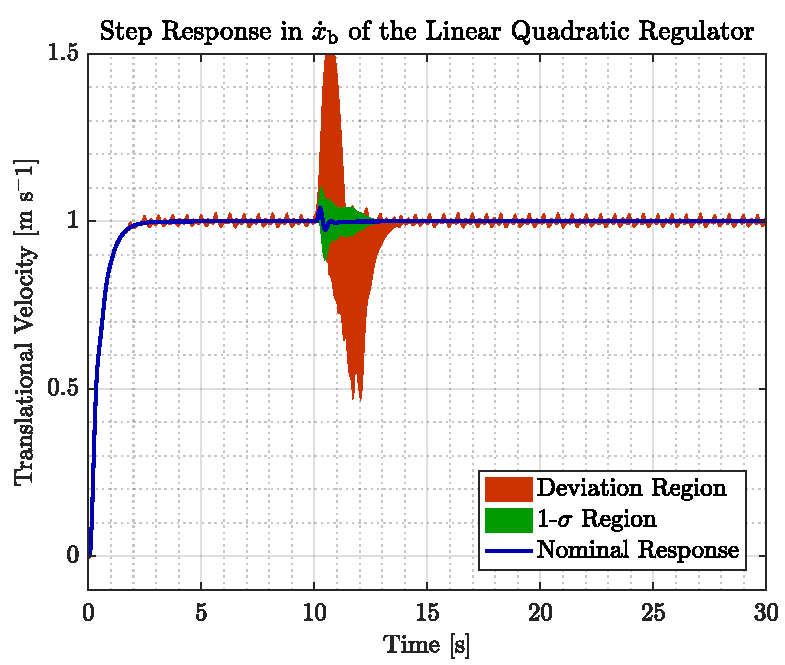
\includegraphics[width=1\linewidth]{figures/xbdot_mc_lqr}
    \end{figure}        
  \end{minipage}\hfill      
  \begin{minipage}{0.45\linewidth}
    \begin{figure}[H]
      \centering
      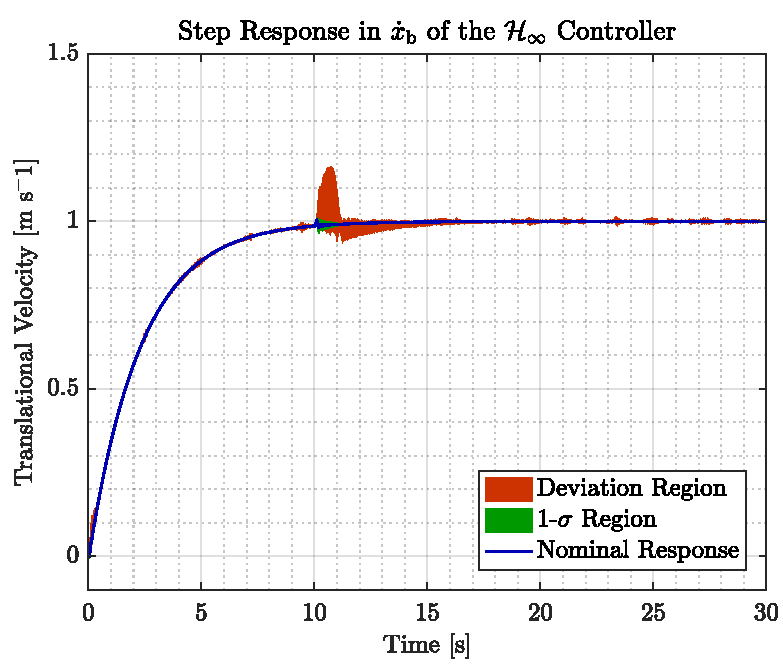
\includegraphics[width=1\linewidth]{figures/xbdot_mc_rob}
    \end{figure}                
  \end{minipage}\hfill \\
\end{figure}
\end{frame}



\begin{frame}{Inner Controller}{Comparison of the Controllers}
  \begin{figure}[H]
    \begin{minipage}{0.45\linewidth}
      \begin{figure}[H]
        \centering
        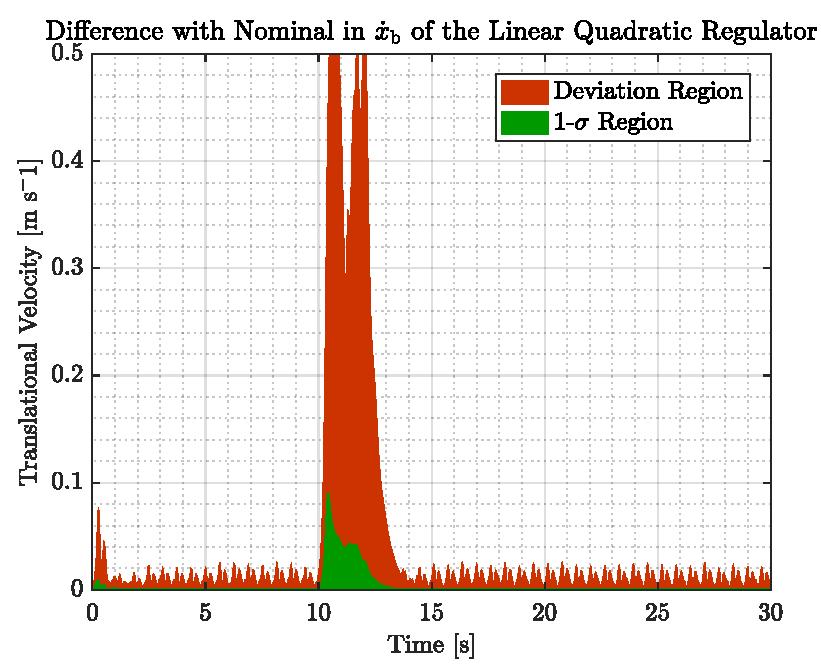
\includegraphics[width=1\linewidth]{figures/xbdot_mc_lqr_error}
      \end{figure}        
    \end{minipage}\hfill      
    \begin{minipage}{0.45\linewidth}
      \begin{figure}[H]
        \centering
        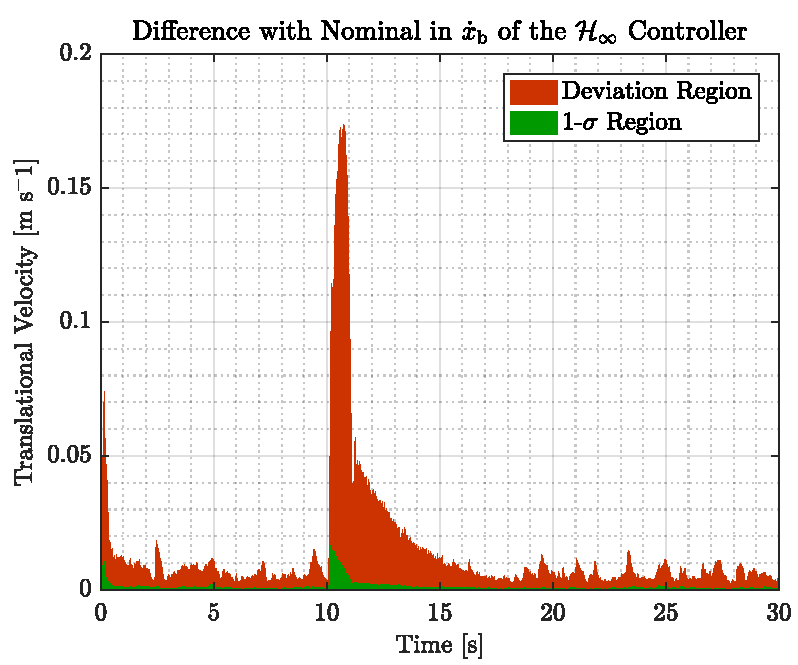
\includegraphics[width=1\linewidth]{figures/xbdot_mc_rob_error}
      \end{figure}                
    \end{minipage}\hfill \\
  \end{figure}
\end{frame}



\begin{frame}{Inner Controller}{Comparison of the Controllers}
  \begin{figure}[H]
    \begin{minipage}{0.45\linewidth}
      \begin{figure}[H]
        \centering
        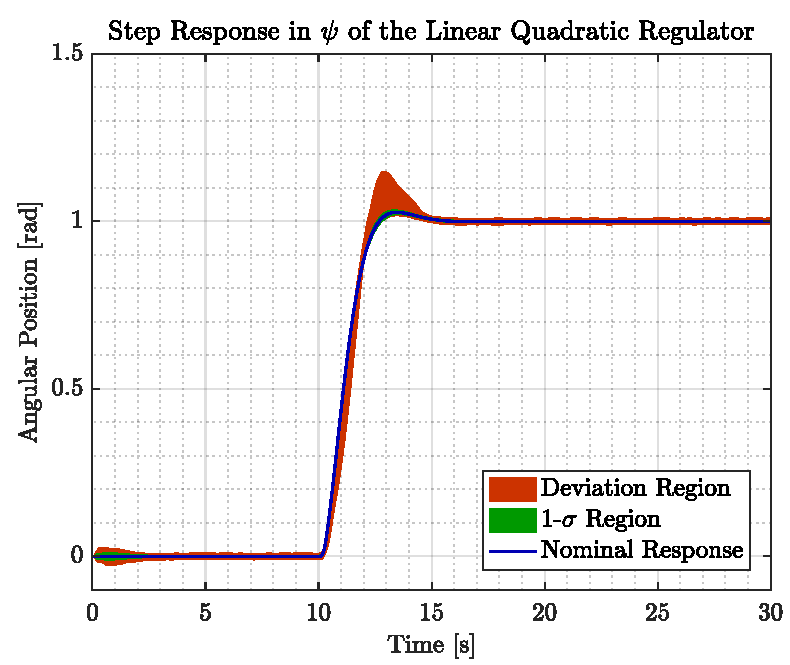
\includegraphics[width=1\linewidth]{figures/yaw_mc_lqr}
      \end{figure}        
    \end{minipage}\hfill      
    \begin{minipage}{0.45\linewidth}
      \begin{figure}[H]
        \centering
        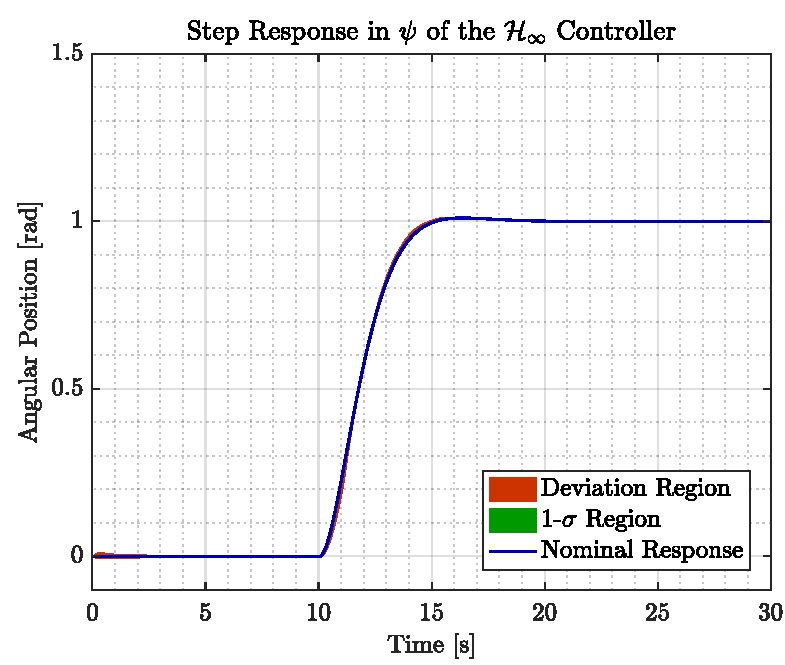
\includegraphics[width=1\linewidth]{figures/yaw_mc_rob}
      \end{figure}                
    \end{minipage}\hfill \\
  \end{figure}
\end{frame}



\begin{frame}{Inner Controller}{Comparison of the Controllers}
  \begin{figure}[H]
    \begin{minipage}{0.45\linewidth}
      \begin{figure}[H]
        \centering
        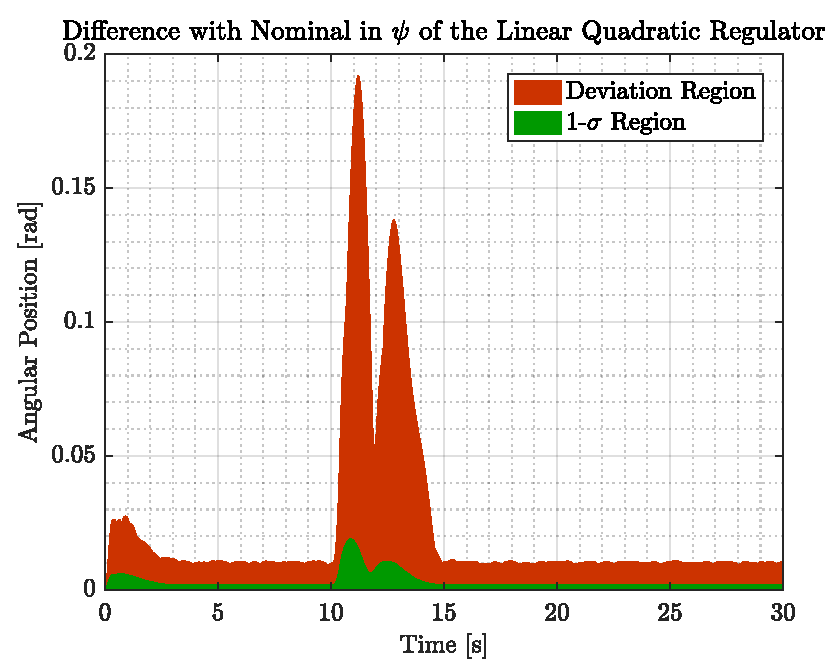
\includegraphics[width=1\linewidth]{figures/yaw_mc_lqr_error}
      \end{figure}        
    \end{minipage}\hfill      
    \begin{minipage}{0.45\linewidth}
      \begin{figure}[H]
        \centering
        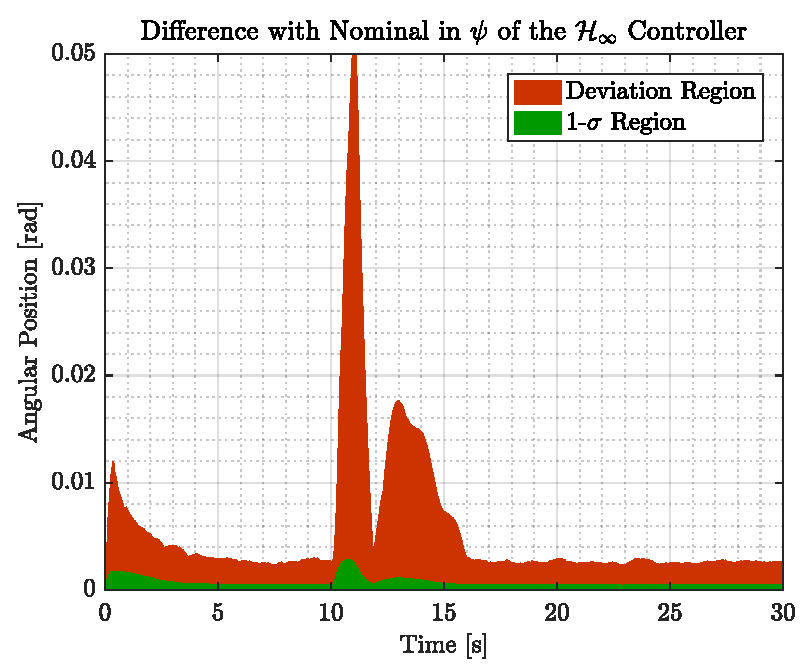
\includegraphics[width=1\linewidth]{figures/yaw_mc_rob_error}
      \end{figure}                
    \end{minipage}\hfill \\
  \end{figure}
\end{frame}

